%!TEX root = ../2019_7_Ozgumus_Semsi_Yigit.tex

\begingroup

%% Anomaly Detectioni anlat abstracten acip
Anomaly detection is an increasingly popular field in computer vision and is a challenging 
problem concerning wide variety of application domains such as cyber security, healthcare, 
finance and Internet of Things (IoT) \cite{Chandola:2009:ADS:1541880.1541882}. Problems encountered
in these areas are tackled with data driven methods in order to ensure reliability for largely scaled 
environments and anomaly detection becomes an important task to control the effectiveness of the data.
Anomalies can be defined as the samples that don't follow the characteristic behaviors 
of the defined notion of normality for that data \cite{Chandola07anomalydetection:}. 
Significance of anomaly detection comes 
from the fact that abnormalities in the data may often be translated to critical and 
actionable information. For example, security system of a data center monitors the anomalies 
in the network traffic and the process use to detect intrusions and unauthorized access \cite{JABEZ2015338,AHMED201619}.
Industrial systems use anomaly detection on the sensory data coming from the equipment to 
monitor the quality and maintenance needs \cite{inproceedings_industry}. 

One of the main problems of solving anomaly detection task is acquiring the data for anomalous cases. 
Depending on the domain, anomaly might be a very rare occurrence or it might be costly for the 
system to replicate the conditions of the anomalous case. 
In such cases where there is an imbalance between the proposition of normal and anomalous 
data in the dataset, reconstruction based methods are very promising option for anomaly detection. 
Reconstruction based methods for anomaly detection focus on computing the representation for 
a normal portion data, and uses this representation to differentiate the normal and anomalous 
samples in the testing dataset. 

In many cases of feature representation problems, high dimensional data such as images lie
in a low dimensional subspace which contains most salient features of the image. Reconstruction 
based methods use this prior for anomaly detection purposes.
Main premise of reconstruction based methods is that performing anomaly detection on higher 
dimensional feature space such as images, as anomalous or normal, becomes easier if the underlying 
normal data lies in a subspace of lower dimensionality than its original form 
\cite{Beyer:1999:NNM:645503.656271}. Hence we can model the normal data in a lower dimensional 
complexity and find an appropriate way to reconstruct to its original higher-dimensional 
representation. Finally defining a score to measure the difference between the normal data and its reconstruction 
provides us a method to detect anomalies. Since the model is trained only with the normal data, 
encoding an anomalous sample to a lower dimensional complexity and then reconstructing using a decoder 
network to its higher dimensional representation would produce a higher score 
than the normal data. Finding a threshold to determine the boundary between the scores 
of normal data samples and anomalous samples depends on the dataset and 
the problem domain.

Autoencoder networks (see Section \ref{sec:ae}) have been heavily used for reconstruction based anomaly 
detection in recent years. They consist of an encoder and decoder network. Encoder 
network is trained to learn the latent representation and decoder network is trained to obtain 
the reconstruction to model the normality of data with no anomalies. Over the years, different 
variants of autoencoder networks are employed for anomaly detection task
\cite{kingma2013autoencoding, Masci2011StackedCA, an2015variational, leveau2017adversarial, Pidhorskyi:2018:GPN:3327757.3327787}. Generative Adversarial Network (GAN) is a relatively new method 
in deep learning that can generate new and unobserved data with unsupervised training. 
It has been used by several models \cite{Donahue2017AdversarialFL,Dumoulin2017AdversariallyLI,DBLP:journals/corr/abs-1812-02288,Akay2018GANomalySA,Akay2019SkipGANomalySC} to investigate its impact for anomaly detection in image data.

\begin{figure}[h!] \subfloat[Normal samples]{
		\begin{minipage}[c][0.8\width]{0.5\textwidth}
			\centering
			\fbox{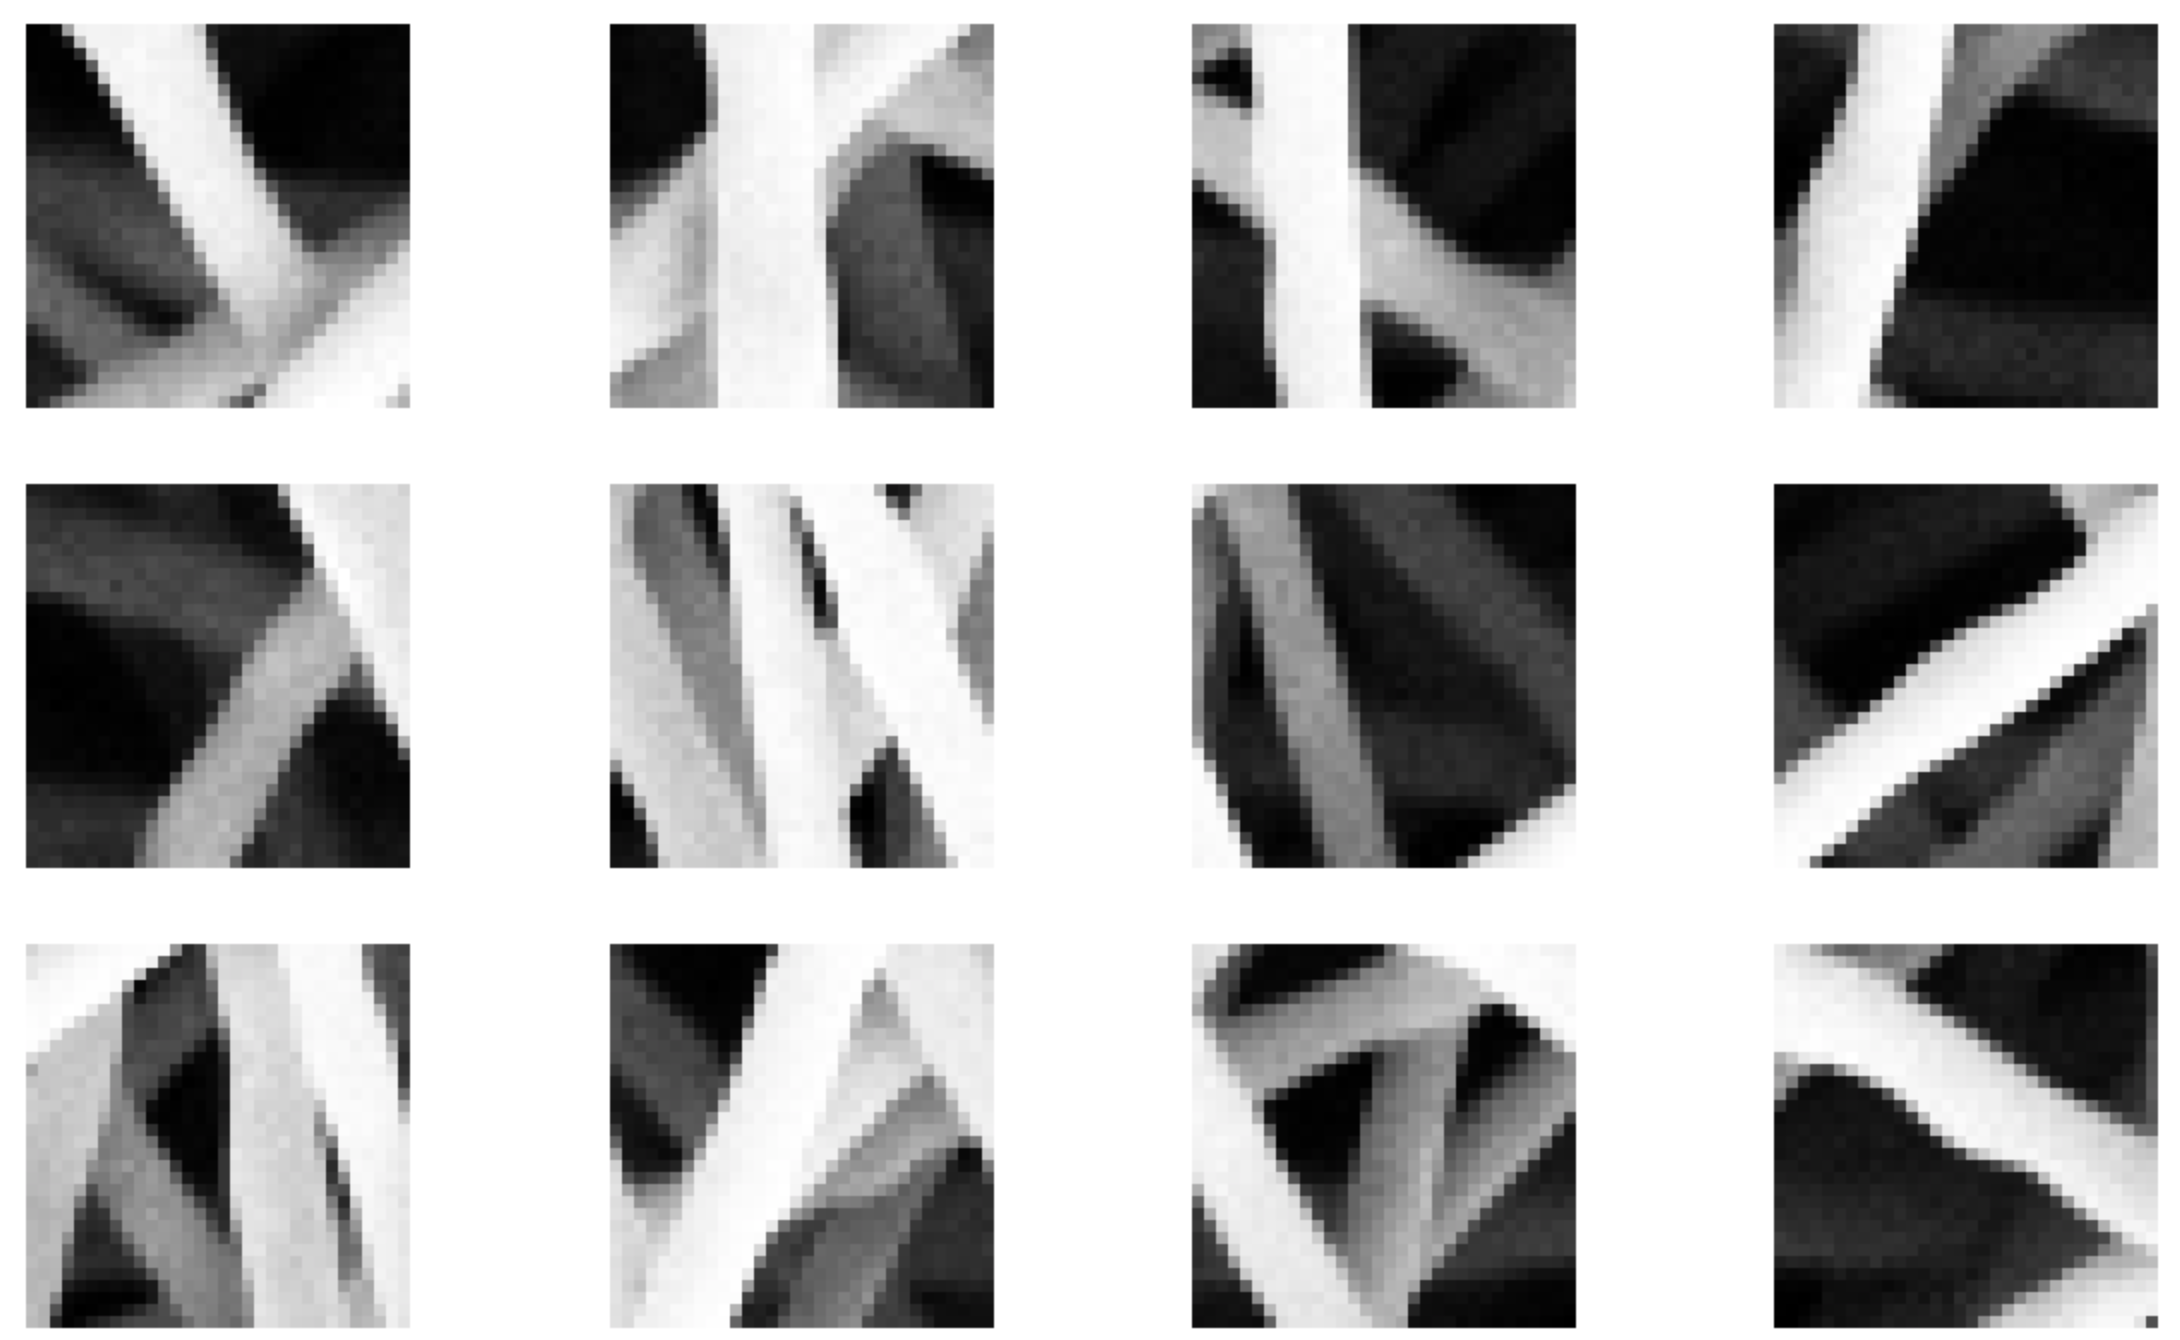
\includegraphics[width=1\textwidth]{sample_normal}}
			\label{fig:data_sample_normal_intro}
	\end{minipage}}
	\hspace*{\fill} \subfloat[Samples with anomalous regions]{
		\begin{minipage}[c][0.8\width]{0.5\textwidth}
			\centering
			\fbox{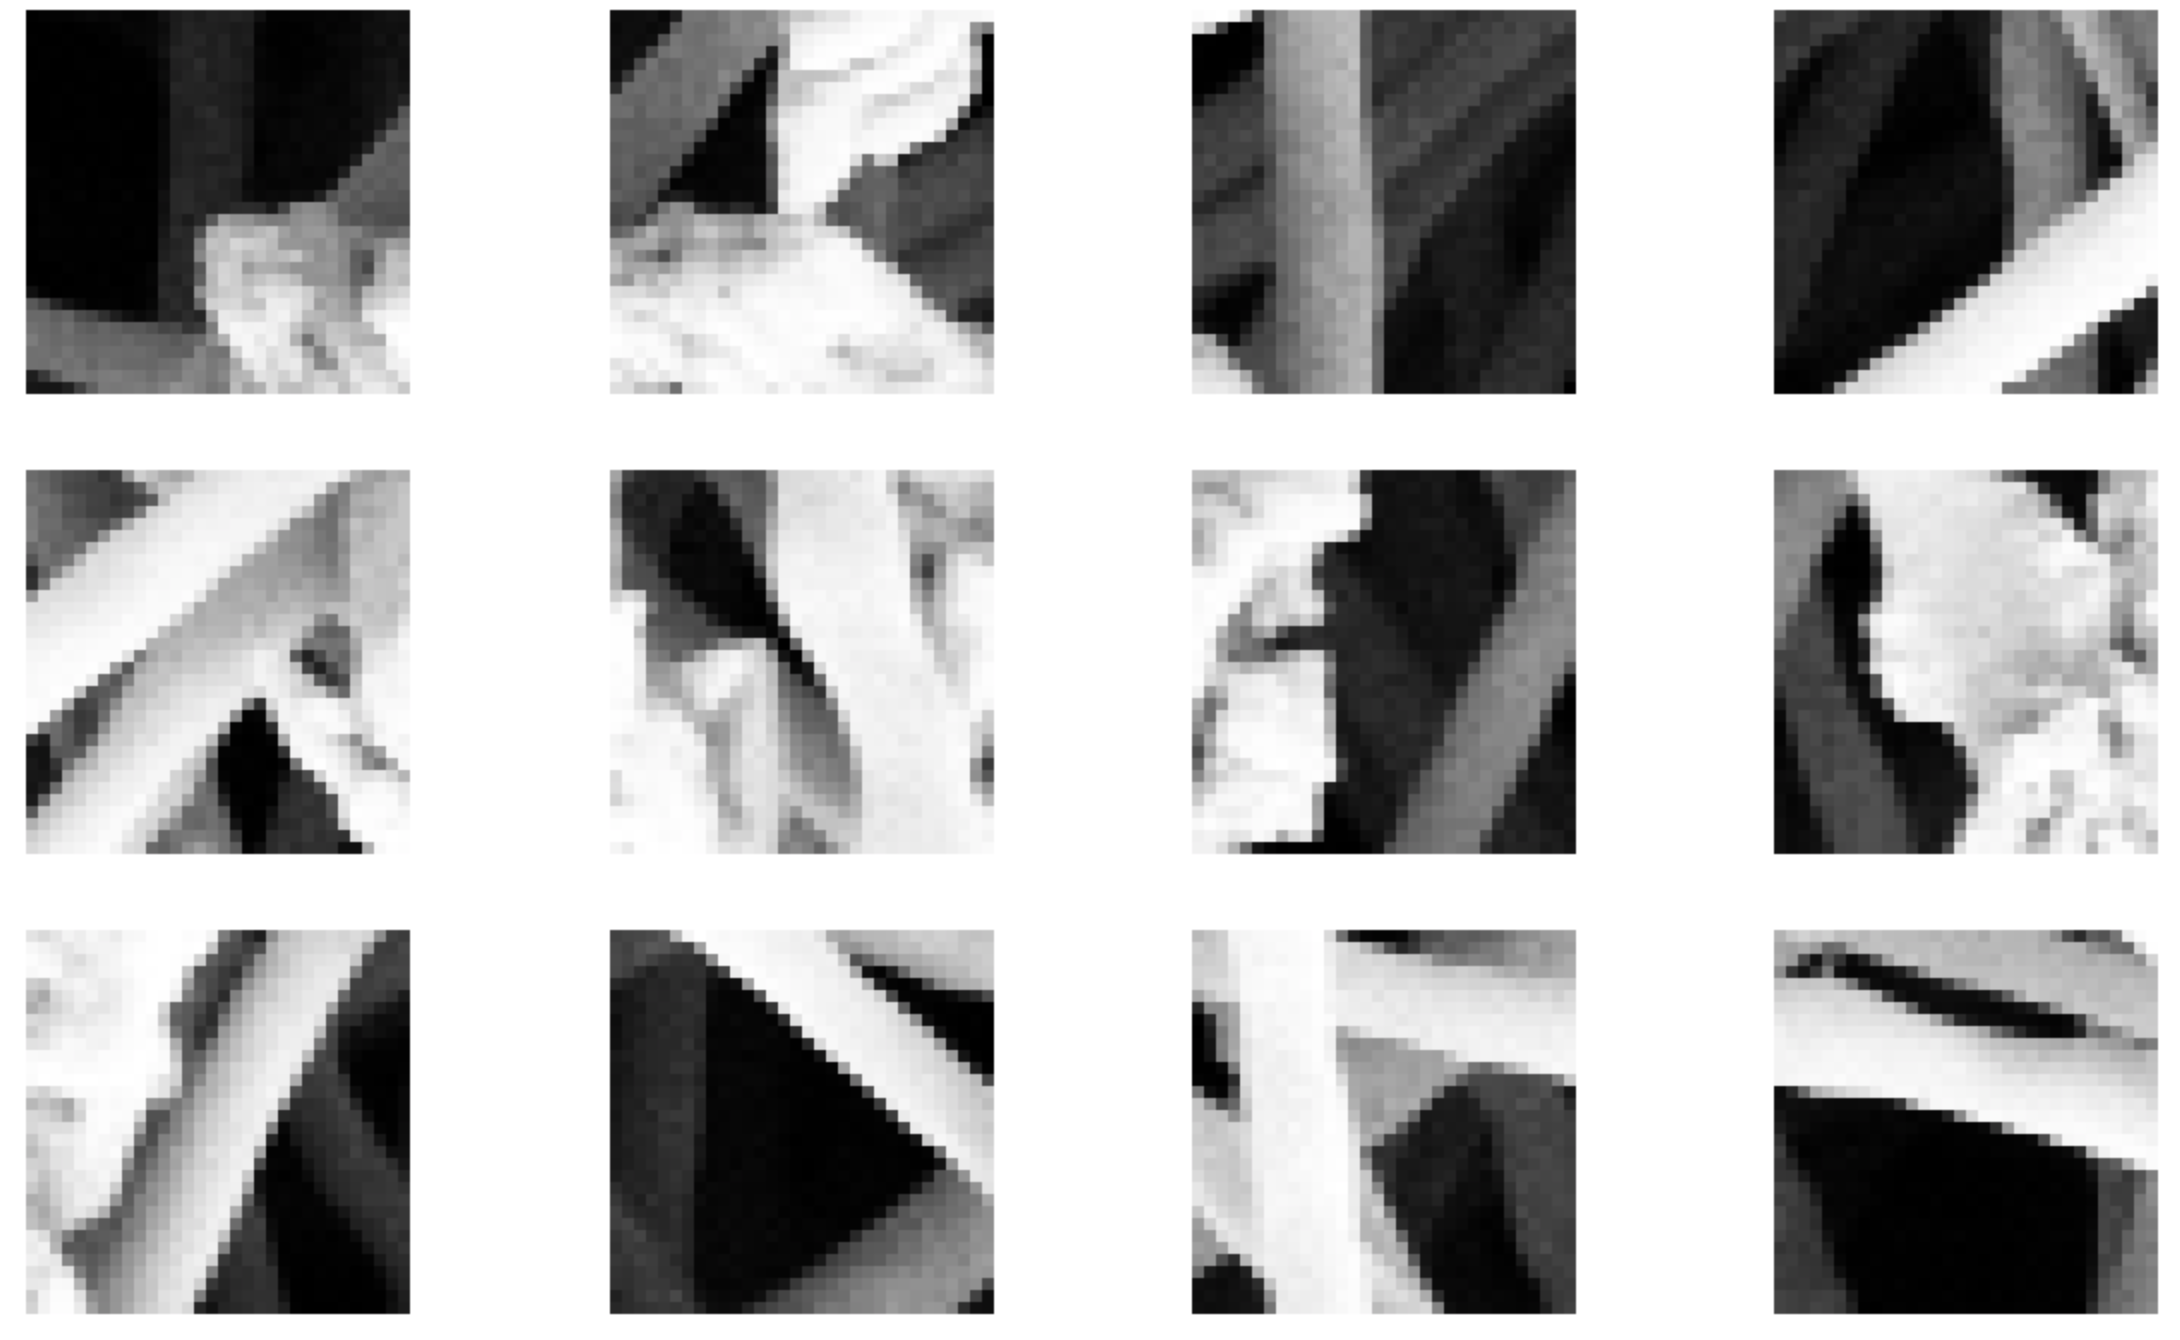
\includegraphics[width=1\textwidth]{sample_anomaly}}
			\label{fig:data_sample_anomaly_ano}
	\end{minipage}}
	\caption{Normal and Anomalous region patches from the SEM image dataset}
	\label{fig:data_samples_intro}
\end{figure}

%% Modeli acikla cozmeye calistigin seyleri anlat
This thesis investigates the anomaly detection using generative adversarial network and its application 
on the Nanofiber production monitoring \cite{sem} (see Section \ref{sec:sem}). SEM images are images from the 
nanofibrous material manufacturing process called electro spinning method \cite{carrera2016defect}.
 Due to the environmental factors and failures related to the instruments, this method may produce 
samples which has defective/ anomalous regions as illustrated in Figure \ref{fig:data_samples_intro}. 
While these anomalous regions have distinguishable features that can easily be spotted by human eye, 
it is difficult to catalogue these anomalous examples 
for detection with automated systems. Main contributing factors are that defective regions can have 
variety of appearence and shape and the formation of fibers also creates to difficulties for detection
since they can overlap and follow different orientations \cite{carrera2016defect}. Main approach to 
this problem is to learn a model describing the manifold of normal regions by using images from the SEM 
dataset that has no defective regions. This model is then used to detect the defective regions 
of a new SEM image sample by disecting the image into overlapping patches, and determining whether 
each patch conforms or not to the learned model.

\begin{figure}[h!]
	\centering
	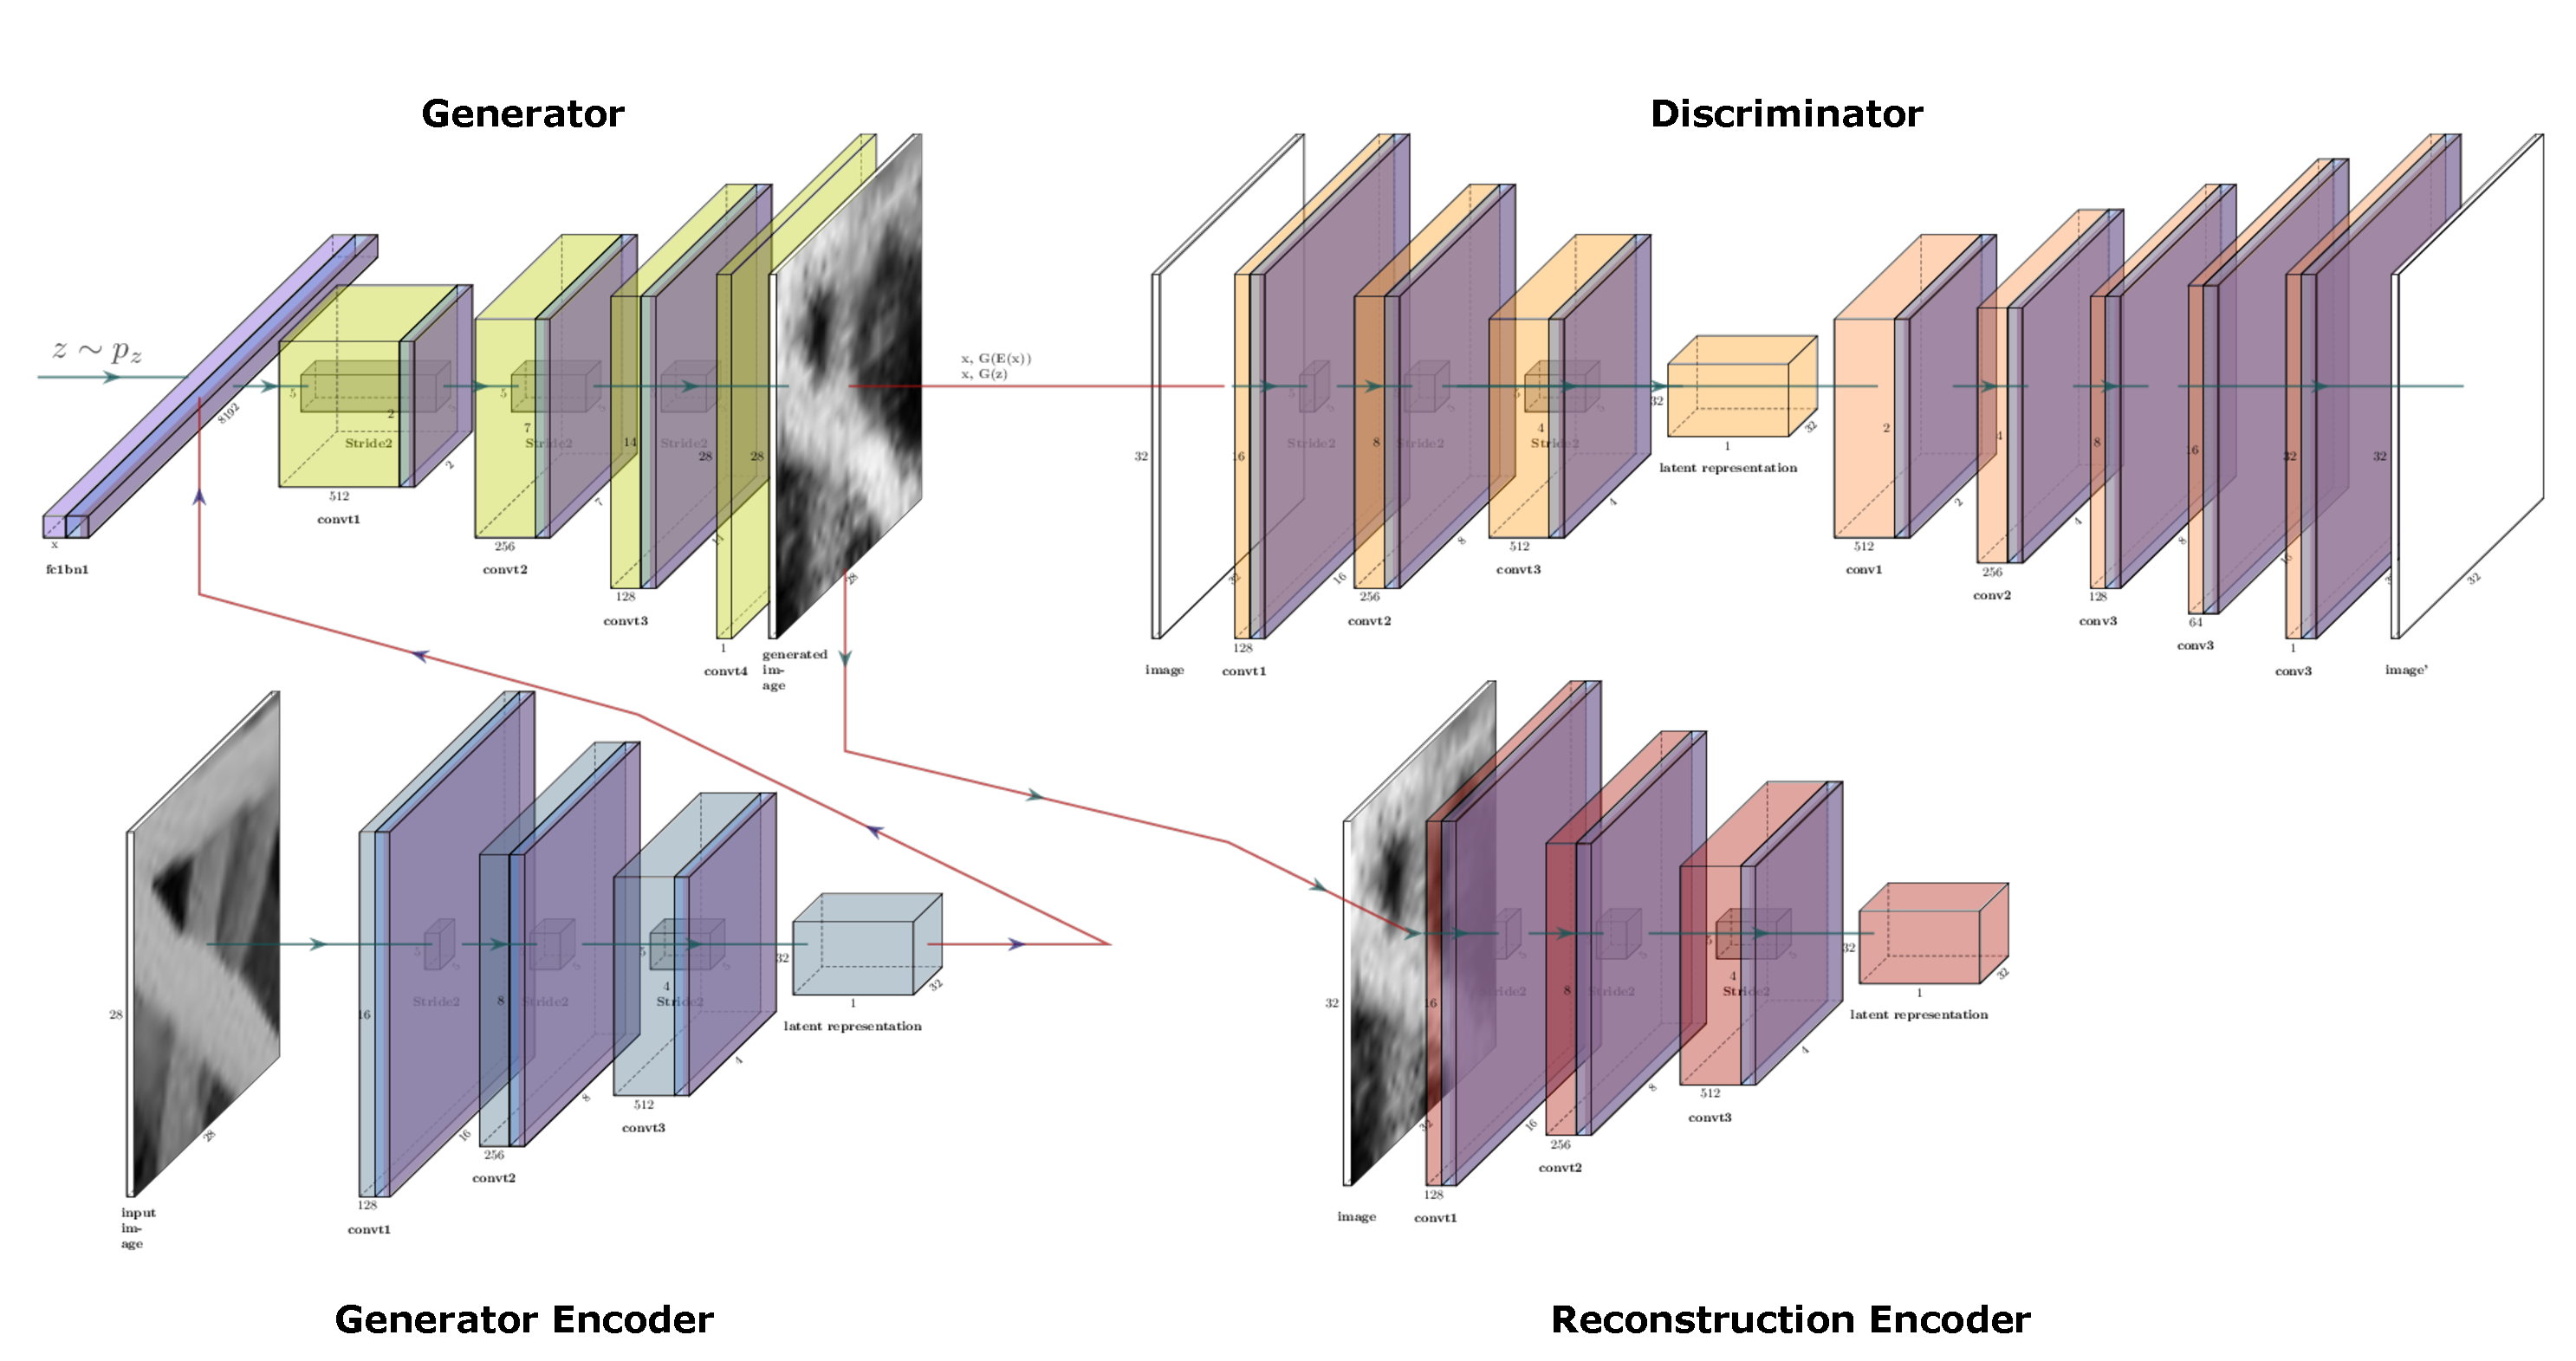
\includegraphics[width=1.0\textwidth]{arim/sencebgan/sencebgan_model}
	\caption{SENCEBGAN Model Overview }
	\label{fig:sencebgan_intro}
\end{figure}

This thesis provides a model that performs a reconstruction based anomaly detection task 
by taking advantage of generative adversarial network and encoder networks on the SEM image dataset.
First part of thesis investigates the performance of anomaly detection methods that utilizes
generative adversarial networks (GAN) (see Section \ref{sec:gan}). Later on a modified model is proposed 
(see Figure \ref{fig:sencebgan_intro}) that addresses the problems encountered in the 
training experiments of GAN based anomaly detection methods. 

Our model uses an energy based generative adversarial network (EBGAN)  (see Section \ref{sec:ebgan}) 
to address the stabilization problems of adversarial training of GAN and two encoder networks to 
learn the latent space  representation of both input images and their reconstructions. Training of the model 
is divided into 3 stages to mitigate the convergence problems of the encoder networks. EBGAN is trained 
in the first stage. Generator encoder network is trained adversarially with generator network of 
EBGAN to learn bidirectional mapping between the image space and latent dimension space in the 
second stage. Then, reconstruction encoder network is trained to learn the latent representation 
of the reconstructed image samples obtained from the generator network. Anomaly detection is performed 
by using an anomaly score computed from the latent representations of the query image and its 
reconstructions. Comparative analysis 
between anomaly detection methods that uses generative adversarial networks and the proposed 
model regarding reconstruction quality of the generator networks and overall performance is carried 
out via an ablation study and a series of incremental experiments (see Chapter \ref{chap:expres}).

Initial experiments of GAN based anomaly detection models show that adversarial training of generator 
and discriminator networks suffer from convergence problems. Ablation study performed with additional 
heuristics for adversarial training provides a small margin of increase in performance but the quality 
and visual similarity of generated images of generator networks suffer greatly from the initial 
adversarial training. Experiment results with energy based GAN exhibit 
more stable training for generator and discriminator networks. Changing the adversarial objective computation 
from log likelihood of probability to a energy based difference provides more stable learning process for GAN 
using SEM image dataset. Experiments for encoder network that is responsible for learning the bidirectional 
mapping between the image and the latent dimension space show that training the network sequentially, after 
GAN training is completed, prevents convergence problems experienced with models that trains their 
generator and encoder network simultaneously. (See BiGAN (Section \ref{sec:bigan}) and 
ALAD ( Section \ref{sec:alad})) Regarding to the reconstruction quality, visual inspection of the 
experiments for reconstructions show that due to the way filaments are structured on top of 
each other, reconstructions of those samples resemble an anomalous sample in certain examples. Experiments 
related to EBGAN show that while the stability is more easily obtained than traditional GAN, improving 
image quality of reconstructions is more difficult and is considered as one of the future 
improvements for this model. Proposition of the secondary encoder network to learn the latent dimension space 
of the reconstructed image samples show promise in improving the overall performance of anomaly detection. 
Experiments with an anomaly detection scores based on the latent representations of the query images and their reconstructions rather than the images itself support the inclusion of the secondary encoder network. In 
general, our model provides a reconstruction based anomaly detection model that utilizes EBGAN and encoder networks.
It also proposes a latent representation based anomaly detection to improve the image based anomaly detection method.


This thesis is organized as follows: Chapter \ref{chap:sota} presents the anomaly detection 
problem thoroughly, introduces the networks that are used for  anomaly 
detection solution such as generative adversarial networks and autoencoder networks and finally 
illustrates mainstream anomaly detection methods that utilize generative adversarial 
networks. Chapter \ref{chap:latdel} introduces some of the latest developments concerning 
GAN and anomaly detection task. Chapter \ref{chap:arim} 
analyzes the problems other GAN based anomaly detection models experience with SEM image dataset 
and presents our proposed model. Experimental results are described in Chapter \ref{chap:expres} 
and the conclusion and the future work are  stated in Chapter \ref{chap:conc}.

\endgroup